\section{Background}
     
A protocol specification can be broken into four components: message format,
initial configuration, state machine, and system interface. Message formats
define the precise structure of a protocol's messages, their contents, and
invariants. The state machine defines the number of unique protocol states 
which an instance of the protocol may be in, along with guarded transition
functions, transition events, and local state manipulation. The configuration
contains the initial parameters required to instantiate a state machine.
Finally, the system interface defines send/receive message passing, time events,
persistent storage, and a general maintenance. This protocol abstraction is
quite useful in reasoning and testing the protocol design in an independent
manner. This work focuses on a network protocol's message format specification.
Specifically, binary message formats common to network protocols from layers 2-4
will be studied.

Binary message formats typically have a self-describing structure called Type
Length Value (TLV). A fixed length type and length field initially indicate the
type of the field to follow. The length usually sets an upper bound on the size
of the following field. This following field may be a single type, a disjoint
union of types, a list of unique type, or a list of disjoint union of types.
This highly variable structure can easily lead to inconsistency, resulting in
unknown behavior without proper message validation. 

\begin{figure}[h]
   \begin{center}
   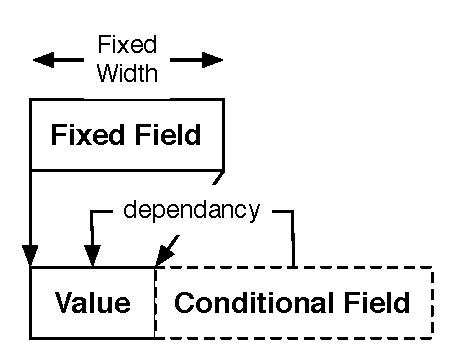
\includegraphics[width=.40\textwidth]{figs/fig1.pdf}
   \caption{Message Format Dependencies}
   \label{figure:fig1}
   \end{center}
\end{figure}

These inconsistencies frequently manifest as vulnerabilities in network protocol
implementations and can be represented by two classes: value constraint, and 
structural constraint violations. A protocol specification might define a subset
of the input range for any particular field, leaving the remainder unspecified,
value constraints are violated when an implementation blindly uses received
values without range validation allowing for undefined behavior. A structural 
constraint violation occurs when a received message describes its structure in
a way that is inconsistent with the message formate specification.
The US-CERT vulnerability database shows these classes of vulnerabilities exist
and are easy to find in current implementations of simple, mature, protocols by
experienced engineers and organizations~\cite{us_cert}. \\
\\
\begin{tabular}{|c|c|c|c|c|}
   \hline
   Age & Protocol & Vendor & Bug Date & US CERT \# \\ \hline
   \hline
   1985 & Bootp & Apple & 2006 & 77628 \\ \hline
   1990 & 802.1q VLAN & Cisco & 2006 & 821420 \\ \hline
   1981 & ICMP & Cisco & 2007 & 341288 \\ \hline
   1985 & NTPD & GNU & 2009 & 853097 \\ \hline
   1998 & OSPFv2 & Quagga & 2012 & 551715 \\ \hline
\end{tabular} \\

At the heart of network protocol message structure is type dependency. Precisely
sized types can depend on the values from previously occurring fields. This 
structure can be captured precisely with a small set of primitive types extended
with dependency.

\subsection{Prior Work}

PacketTypes~\cite{packet_types} is a first work towards developing a
language to handle the specific constraints of network protocol
message formats. The authors' motivate the work with the usual suspects
of networkk protocol software development: tedious, error-prone, ever-changing,
etc. Users can specific binary formatted network protocols in the PacketTypes
overlay language. This language is then compiled down to a set of C
datastructures and functions. Type checking is performed at the overlay level,
while runtime checks are provided through their generated C functions.

DataScript~\cite{datascript} is an overlay language designed to provide
declarative ad-hoc data format specifications. This work aimed to advance the
work of PacketTypes for more general data formats as well as generate
traversal functions for verified data. This language targeted the Java
runtime environment.

Binpac~\cite{binpac} can be viewed as an extension of
PacketTypes~\cite{packet_types}, the authors' primary view is that
protocol message formats are merely a grammar problem, and seek
to generalize a format description language into a `data-model' with
constraints. The problem is described in the same terms as with PacketTypes:
tedious, error-prone, hard-to-read, etc. The generalization includes support for
ASCII based protocols which was not present with previous
work~\cite{packet_types}. The target application is off-line packet capture
analysis.

PADS~\cite{pads_orig} is a declarative overlay implemented for: C, ML, and
Haskell as a work in progress. The goal for PADS is to capture the richness
of ad-hoc data formats: ASCII, binary, Cobol, and `mixed data formats.' The
targeted user of the PADS system are system administrators who deal with large
variations and constant change of ad-hoc data formats. The authors give many
examples detailing various XML and log file processing requirements of network
service providers.

PADS/ML~\cite{pads_ml} is the most relevant work related to Steve. Steve 
differs from PADS/ML in the following ways. First, Steve is targeting on-line
network protocol design, verification, and implementation; while PADS/ML
targets off-line ad-hoc data format processing. Steve integrates the network
protocol specification within the host language to allow compile time reasoning
about correct usage of messages. PADS/ML provides an overlay language for format
specification, type-checks a specification for consistency, and then generates a
library in the host language for use. By embedding the message format 
specification in the host language Steve is able to capture value and structural
constraint violations from format definition and usage at compile time.
